\newcommand{\vect}[1]{\mathbf{#1}}

\item \points{12} {\bf AdaBoost}

Consider building an ensemble of decision stumps $f_t$ with the AdaBoost algorithm,
$$F(x) = \text{sign}\Big(\sum_{t=1}^T \hat{w}_t f_t(x)\Big).$$
Figure~\ref{fig:adaboost} displays a 2-dimensional training dataset, as well as the first stump chosen. A stump predicts binary $+1 / -1$ values, and depends only on one coordinate value (the split point). The little arrow indicates the positive side where the stump predicts $+1$. All points start with uniform weights.
\begin{figure}[ht]
	\centering
	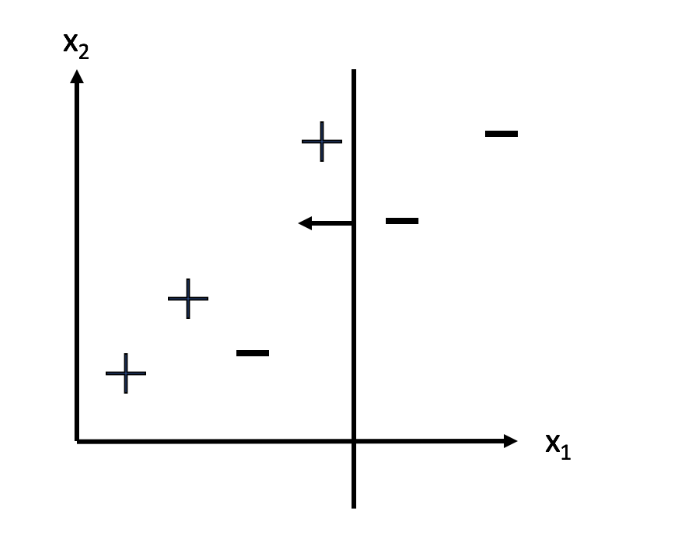
\includegraphics[width=0.45\linewidth]{adaboost/fig6-decision-boundary.png}
	\vspace{-0.1in}
	\caption{2-dimensional labeled data, where `+' corresponds to class $y=+1$ and `-' corresponds to class $y = -1$. The decision boundary for the first decision stump is shown.  The arrow points in the positive direction from this decision boundary.}
	\label{fig:adaboost}
\end{figure}

\begin{enumerate}
    \item \subquestionpoints{3} Given a set of $n$ observations $(x_i, y_i)$ where $y_i$ is the label $y_i \in \{-1,1\}$, let $f_t(x)$ be the weak classifier at step $t$ and let $\hat{w}_t$ be its weight. First we note that the final classifier after $T$ steps is defined as
		\begin{align*}
			F(x) = \text{sign} \left\{\sum_{t=1}^T \hat{w}_t f_t(x) \right\}
			= \text{sign}\{f(x)\},
		\end{align*}
	where
	\begin{align*}
		f(x) = \sum_{t=1}^T \hat{w}_t f_t(x).
	\end{align*}
	We can assume that $f(x)$ is never exactly zero.

	Show that
	\begin{align*}
		\varepsilon_{\text{training}}
		:= \frac{1}{n} \sum_{i=1}^n 1_{\{F(x_i) \neq y_i\}}
		\le \frac{1}{n} \sum_{i=1}^n \exp(-f(x_i) y_i),
	\end{align*}
	where $1_{\{F(x_i) \neq y_i\}}$ is $1$ if $F(x_i) \neq y_i$ and $0$ otherwise.
    
	\ifnum\solutions=1 {
	\begin{answer}
\newpage
\end{answer}
        } \fi
        
    \item \subquestionpoints{5} List out the cases where Gini loss will stay the same after a split.  Show why these do not violate the strong concavity of the Gini loss.  Briefly explain why these cases do not prevent a fully grown tree from achieving zero Gini loss. (\textbf{Hint}: Recall the definition of strict concavity).
    
	\ifnum\solutions=1 {
	\begin{answer}
\newpage
\end{answer}
        } \fi
        
    \item \subquestionpoints{4} Will the second stump receive higher coefficient in the ensemble than the first? In other words, will $\hat{w}_2 > \hat{w}_1$? Briefly explain your answer. (No calculation should be necessary.)
    
	\ifnum\solutions=1 {
	\begin{answer}
\newpage
\end{answer}
        } \fi
        
\end{enumerate}
